% !TEX root = ../main.tex

\begin{figure}[t]
\centering
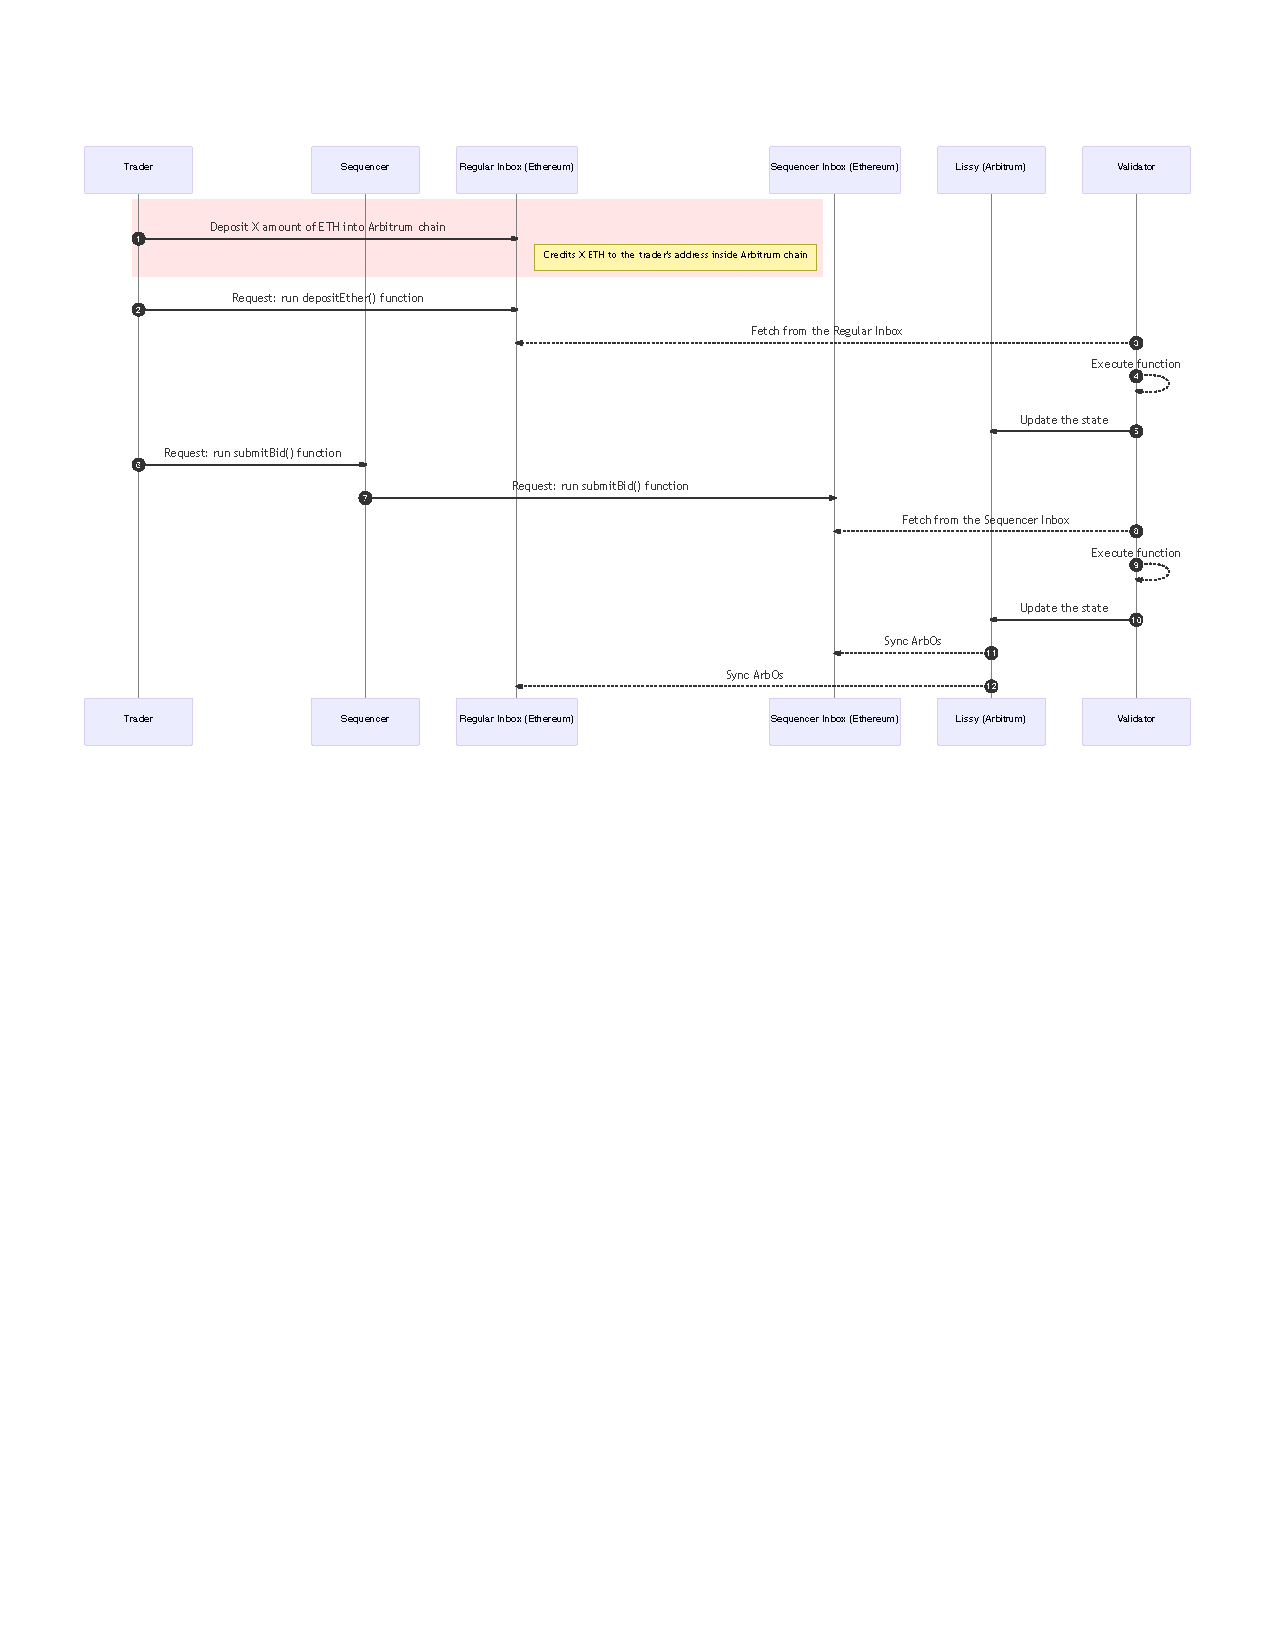
\includegraphics[width=1\textwidth]{fig/lissyL2.pdf}
\caption{\footnotesize{\cm L2 Diagram}  \label{fig:lissyl2}}
\end{figure}

\textbf{Ethereum's Gas Model.} Every transaction results in the participating nodes having to execute bytecode. This is not free. When a transaction is executed, each opcode in the execution path accrues a fixed, pre-specified amount of \emph{gas}. The function caller will pledge to pay a certain amount of Ethereum's internal currency \emph{ETH} (typically quoted in units of Gwei which is one billionth of an ETH) per unit of gas, and miners are free to choose to execute that transaction or ignore it. The function caller is charged for exactly what the transaction costs to execute, and they cap the maximum they are willing to be charged (\textit{gas limit}). If the cap is too low to complete the execution, the miner keeps the Gwei and \emph{reverts} the state of the EVM (as if the function never ran).

A miner can include as many transactions (typically preferring transactions that bid the highest for gas) that can fit under a pre-specified \textit{block gas limit}, which is algorithmically adjusted for every block. As of the time of writing, the limit is approximately 11M gas. Essentially, our main research question is how many on-chain trades can be executed without exceeding that limit. Later, we also discuss several bytecode operations (\emph{opcodes}) that refund gas (\ie cost negative gas), which we heavily utilize in our optimizations.


\section{Gas Refunds.} In order to reconstruct the current state of Ethereum's EVM, a node must obtain a copy of every variable change since the genesis block (or a more recent `checkpoint' that is universally agreed to). For this reason, stored variables persist for a long time and, at first glance, it seems pointless to free up variable storage (and unclear what `free up' even means). Once the current state of the EVM is established by a node, it can forget about every historical variable changes and only concern itself with the variables that have non-zero value (as a byte string for non-integers) in the current state (uninitialized variables in Ethereum have the value 0 by default). Therefore, freeing up variables will reduce the amount of state Ethereum nodes need to maintain going forward.

For this reason, some EVM operations cost a negative amount of gas. That is, the gas is refunded to the sender at the end of the transaction, however (1) the refund is capped at 50\% of the total gas cost of the transaction, and (2) the block gas limit applies to the pre-refunded amount (\ie a transaction receiving a full refund can cost up to 5.5M gas with an 11M limit). Negative gas operations include:

\begin{itemize}

\item \texttt{SELFDESTRUCT}. This operation destroys the contract that calls it and refunds its balance (if any) to a designated receiver address. The  \texttt{SELFDESTRUCT} operation does not remove the initial byte code of the contract from the chain. It always refunds 24,000 gas. For example, if contract A stores a single non-zero integer and contract B stores 100 non-zero integers, the \texttt{SELFDESTRUCT} refund for both is the same (24,000 gas).


\item \texttt{SSTORE}. This operation loads a storage slot with a value. Using \texttt{SSTORE} to load a zero into a storage slot means the nodes can start ignoring it (recall that all variables, even if uninitialized, have zero by default). Doing this refunds 15,000 gas per slot.

\end{itemize}







\section{Roll-ups: Additional Background}
\label{app:rollup}



We have avoided augmenting \cm with centralized components and third party services as our research question concerns the feasibility of a system with a minimum of regulatory hooks. However from a regulatory stance, there is a big difference between an architecture where the centralized component is publicly visible and interacted with by users (\eg most DEXes, roll-up architectures like Loopring, and commit-chain solutions like TEX). We consider an alternative design that is almost as difficult to regulate as a fully on-chain solution. In this design, an off-chain component is introduced to boost performance but it only interacts with the Ethereum network and never directly with traders. Traders still only interact with Ethereum.


\textit{Layer 2} solutions are a group of technologies that are designed and proposed to address specific drawbacks of executing transactions on \textit{Layer 1} (\ie Ethereum and other blockchains)~\cite{gudgeon2020sok}. These technologies focus on fast transaction throughput, reducing gas costs, or educing transaction latency. When using \cm, we strive to reduce the gas cost as performance is the main bottleneck. Thus, we choose a Layer 2 technology called \textit{roll-up} which aims at reducing the gas cost for operating on Layer 1 by taking the transaction executions off-chain and only using the Ethereum blockchain for storing data. In a roll-up, every transaction is executed by a server or cluster of servers known as \textit{validators} that can be run by a collection of users or third party operators (here they can be run by the token issuer). These validators then push the result of the executions (\ie updates in the EVM state) back to the Ethereum and assure the Ethereum network that the transactions have been executed correctly.


A function can be computed off-chain and the new state of the DApp, called a \textit{rollup}, is written back to the blockchain, accompanied by either (1) a proof that the function was executed correctly, or (2) a dispute resolution process that can resolve, on-chain, functions that are not executed correctly (\eg Arbitrum~\cite{kalodner2018arbitrum}). In the case of (1), validating the proof must be cheaper than running the function itself. There are two main approaches: (1a) the first is to use cryptographic proof techniques (\eg SNARKS~\cite{BCGTV13,GGPR13} and variants~\cite{BBHR19}). This is called a \textit{zk-rollup}. Note that the proofs are heavy to compute (introducing a burden to the validators who generate them) but considered valid once posted to the Ethereum. The second approach (1b) is to execute the function in a trusted execution environment (TEE; \eg Intel SGX) and validate the TEE's quote on-chain (\eg Ekiden~\cite{cheng2019ekiden}).\footnote{The TEE-based approach is mired by recent attacks on SGX~\cite{SGX1,SGX2,SGX3,SGX4}, however these attacks do not necessarily apply to the specifics of how SGX is used here, and safer TEE technologies like Intel TXT (\cf~\cite{ZBC+19}) can be substituted.} Approach (2) is called an \textit{optimistic roll-up}. Although the dispute time delays result in a slower transaction finality, optimistic roll-ups substantially increase the performance by decreasing the gas cost.


\section{Cleaning Up Revisited}
\label{app:clean}

Beyond the cleaning up issues with priority queues in Section~\ref{sec:gasrefund}, \textblue{\cm also uses mappings with each market}. Traders preload their account with tokens to be traded (which comply with a common token standard called ERC20) and/or ETH. \cm tracks what they are owed using a mapping called \texttt{totalBalance} and allows traders to withdraw their tokens at any time. However if a trader submits an order (\ie ask for their tokens), the tokens are committed and not available for withdrawal until the market closes (after which, the balances are updated for each trade that is executed). Committed tokens are also tracked in a mapping called \texttt{unavailableBalance}. Sellers can request a token withdrawal up to their total balance subtracted by their unavailable balance.

As the DApp runs \texttt{closeMarket()}, it starts matching the best bids to the best asks. As orders execute, \texttt{totalBalance} and \texttt{unavailableBalance} are updated. At a certain point, the bids and asks will stop matching in price. At this point, every order left in the order book cannot execute (because the priority queue sorts orders by price, and so orders deeper in the queue have worst prices than the order at the head of the queue). Therefore all remaining entries in \texttt{unavailableBalance} can be cleared.

In Solidity, it is not possible to delete an entire mapping without individually zeroing out each entry key-by-key. At the same time, it is wasteful to let an entire mapping sit in the EVM when it will never be referenced again. The following are some options for addressing this conflict.

\begin{enumerate}

\item \textbf{Manually Clearing the Mapping.} Since mappings cannot be iterated, a common design pattern used by DApp developers is to store keys in an array and iterate over the array to zero out each mapping and array entry. Clearing a mapping this way costs substantially more to clear than what is refunded.

\item \textbf{Store the Mapping in a Separate DApp.} We could wrap the mapping inside its own DApp and when we are done with the mapping, we can run \texttt{SELFDESTRUCT} on the contract. This refunds us 24,000 gas which is less than the cost of deploying the extra contract. Additionally, every call to the mapping is more expensive because (1) it is an external function call, and (2) the calls need access control to ensure only the market contract can write to it (if a mapping is a local variable, you get private access for free). 

\item \textbf{Leave and Ignore the Mapping.} The final option is to not clear the mapping and just create a new one (or create a new prefix for all mapping keys to reflect the new version of the mapping). Unfortunately, this is the most economical option for DApp developers even if it is the worst option for Ethereum nodes. 

\end{enumerate}

Clearing storage is important for reducing EVM bloat. The Ethereum refund model should be considered further by Ethereum developers to better incentivize developers to be less wasteful in using storage. 